\section{Насколько это важно на реальной сетке}\label{sec:mesh}

Наша работа по восстановлению кривизны~\cite{davis-rtc} измеряет $SU(2)$-силу на сетках гомологической
сферы Пуанкаре при связности Леви-Чивиты метрики Берже. Её нативное действие~--- энергия
хорды: дефект каждой грани равен $D=U_f-1$. В таблице~\ref{tab:angles} приведены углы граней $a$
на этих сетках (\texttt{face\_angles.py}, по зафиксированным входным данным), а
на рис.~\ref{fig:faces} показаны их распределения.

\begin{table}[h!]\centering\small
\caption{Углы голономии граней на сетках $SU(2)$ с метрикой Берже и относительный разрыв между
энергией хорды и энергией дуги при наибольшем угле, $a^2/12$.}
\label{tab:angles}
\begin{tabular}{rrrrr}\toprule
$n$ & число граней & медиана $a$ & макс. $a$ & разрыв энергий хорды и дуги при макс. \\ \midrule
1 & 480 & 0.0684 & 0.0937 & $7.3\times10^{-4}$ \\
2 & 3{,}840 & 0.0172 & 0.0250 & $5.2\times10^{-5}$ \\
3 & 12{,}960 & 0.0076 & 0.0113 & $1.1\times10^{-5}$ \\
5 & 60{,}000 & 0.0027 & 0.0041 & $1.4\times10^{-6}$ \\
\bottomrule\end{tabular}
\end{table}

\begin{figure}[t]\centering
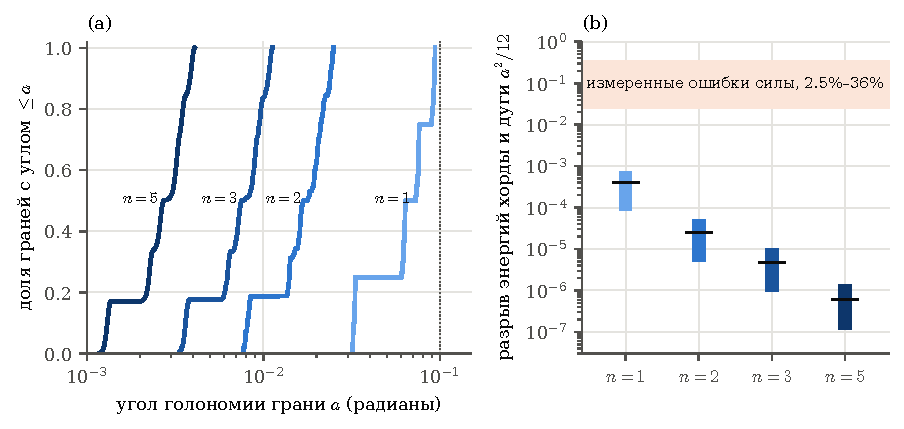
\includegraphics[width=\linewidth]{figures/fig_face_angles.pdf}
\caption{Углы граней на сетках $SU(2)$ с метрикой Берже по зафиксированным входным данным (числа
таблицы~\ref{tab:angles}; \texttt{make\_figures.py} проверяет, что они совпадают). \textbf{(a)}
Функция распределения углов голономии граней на каждом уровне; каждая грань поворачивается менее
чем на $0.1$ радиана. \textbf{(b)} Разрыв энергий хорды и дуги $a^2/12$ по граням: отрезок тянется
от наименьшей грани до наибольшей, а засечка отмечает медиану. Затенённая полоса~--- диапазон
ошибок силы, измеренных на тех же сетках. Разрыв лежит ниже неё на два--пять
порядков.}
\label{fig:faces}
\end{figure}

Углы убывают примерно как площадь грани, а разрыв энергий хорды и дуги всюду меньше
$0.08\%$. Измеренные там ошибки силы составляют от $2.5\%$ до $36\%$. Поэтому
выбор между хордой и дугой не является тем, что ограничивает эту работу, и два используемых там
прочтения (дуга, через $\log U$, для ковариантного восстановления; хорда, $U-1$, для силы)
согласуются с запасом в пределах измеренной ошибки. Где три пути действительно важны для этой
программы, так это во времени: на её самом мелком уровне поток продвигается шагами по правилу Кэли из
раздела~\ref{sec:time}.

\begin{plain}
На сетках, которыми мы на самом деле пользуемся, каждая грань поворачивается меньше чем на десятую
долю радиана. Там короткий путь напрямик и истинный путь различаются по энергии меньше чем на
десятую долю процента, что гораздо меньше ошибок, которые мы измеряем. Так что эта идея не
объясняет те ошибки, и мы говорим об этом прямо. Где она действительно важна, так это в том, как
продвигать движение во времени шаг за шагом, и теперь в той работе для этого используется шаг Кэли.
\end{plain}

\section{Вычисление в GIGI}\label{sec:gigi}

Числа этой статьи находятся в двух местах, и важно, что где. Некоторые из
трёх путей уже входят в GIGI~--- геометрический движок с открытым исходным кодом, в котором
работает наше восстановление кривизны (PolyForm Noncommercial 1.0.0,
\url{https://github.com/nurdymuny/gigi}). Другие пока существуют только в проверочном
скрипте этой статьи. Таблица~\ref{tab:gigi} показывает, что где. Пути указаны относительно корня
репозитория на коммите \texttt{442c13d} ветки \texttt{feat/reading-the-curve}.

\begin{table}[h!]\centering\small
\caption{Где находится каждая идея статьи. «Движок» означает нативный Rust в GIGI;
«скрипт» означает Python в этом каталоге или в \texttt{scripts/} репозитория.}
\label{tab:gigi}
\begin{tabular}{>{\raggedright\arraybackslash}p{4.3cm}>{\raggedright\arraybackslash}p{6.7cm}>{\raggedright\arraybackslash}p{2.2cm}}\toprule
Идея & Где & Вид \\ \midrule
Поворот как число, $q_0=\cos a=\tfrac12\operatorname{Re}\operatorname{tr}U$ &
  примитив \texttt{PLAQUETTE}, \path{src/gauge/plaquette.rs}, одно $q_0$ на грань & движок \\
Половина хорды и сходство, $1-S=d^2=(1-\cos\theta)/2$ &
  \texttt{chord\_d\_sq}, \path{src/dials.rs} & движок \\
Энергия хорды, $D=U_f-1$, взвешенная массой грани &
  \texttt{cell\_action}, \path{src/gauge/ricci_simplicial.rs} & движок \\
Точные связи (перенос вдоль дуги) в метрике Берже &
  \texttt{levi\_civita\_link}, \path{src/gauge/ricci_link.rs} & движок \\
Дуга как отображение, $\exp$ на $\mathfrak{su}(2)$ &
  экспонента Родрига, \path{src/gauge/lie_exp.rs} & движок \\
Шаги по времени &
  \texttt{SYMPLECTIC\_FLOW}: схема чехарды вида «толчок~--- дрейф~--- толчок», дрейф в которой задаётся этой экспонентой,
  \path{src/gauge/symplectic_flow.rs} & движок \\
Углы граней из таблицы~\ref{tab:angles} &
  \texttt{face\_angles.py}, по выходным данным \path{examples/ricci_operator_probe.rs} &
  скрипт на выходе движка \\
Энергия дуги (Мантона), энергия касательной, смесь $2{:}1$ &
  \texttt{verify.py} & скрипт \\
Отображение Кэли и шаг Кранка~--- Николсон & \texttt{verify.py}; на сетке~--- \path{scripts/ricci_su2_pg_flow_cayley.py} & скрипт \\
Сходство по Хаару и Бертран & \path{scripts/haar_sameness.py}, \texttt{verify.py} & скрипт \\
\bottomrule\end{tabular}
\end{table}

\paragraph{Хорда, как её вычисляет движок.} Исходное $SU(2)$-действие из
раздела~\ref{sec:mesh}~--- это в точности энергия хорды. Голономия каждой грани составляется из её
трёх связей, и из её скалярной части вычитается единица:
\begin{lstlisting}[style=rust]
let (a, b, c) = [(0, 3, 1), (0, 4, 2), (1, 5, 2), (3, 5, 4)][face];
let mut h = product(product(u[a], u[b]), inverse(u[c]));
h[0] = h[0] - Jet::constant(1.);      // the chord: D = U_f - 1
...
energy = energy + Jet::constant(2. * mass[(i, j)]) * defects[i][k] * defects[j][k];
\end{lstlisting}
Переменные~--- джеты прямого режима, поэтому тот же проход точно возвращает все восемнадцать
правотривиализованных производных. Углы граней из таблицы~\ref{tab:angles} считаны с того, что этот
код выдал на зафиксированных сетках: нативный зонд \path{examples/ricci_operator_probe.rs},
собранный из приведённого выше исходного кода, исполняемый файл которого закреплён в квитанциях той работы его
SHA-256 (\texttt{71fb30db\ldots}).

\paragraph{Движок шагает вдоль дуги, а не по касательной.} Интегратор GIGI,
\texttt{SYMPLECTIC\_FLOW}, сдвигает каждую связь экспоненциальным отображением, то есть по дуге,
схемой чехарды вида «толчок~--- дрейф~--- толчок», управляемой силой Вильсона. Исследовательский поток
работы по восстановлению кривизны~\cite{davis-rtc} использует метод Рунге~--- Кутты~--- Мунте-Кааса
четвёртого порядка, также построенный на экспоненте, а на самом мелком уровне~--- шаг Кэли из
раздела~\ref{sec:time} (\path{scripts/ricci_su2_pg_flow_cayley.py}). Там шаг был
проверен перед использованием: его отклонение от экспоненты убывает как $|v|^3/12$, его порядок по
времени равен $1.99$, и восемь шагов воспроизводят прогоны четвёртого порядка с точностью до $1.5\%$,
затрачивая от пятой до третьей части вычислений силы. Это исследовательский скрипт. В самом движке
шаг Кранка~--- Николсон пока остаётся предложением, а не описанием.

\paragraph{Чего нет в движке.} Энергия дуги (Мантона), энергия касательной и
комбинация из предложения~\ref{prop:energy} вычисляются только в \texttt{verify.py}. Ни одна из них
не является глаголом движка, и ни одна не проверялась внутри моделирования. Шаг Кэли проверялся, в
описанном выше исследовательском потоке, но и он не является глаголом движка.

\begin{plain}
Часть этой статьи уже есть внутри движка, которым мы пользуемся: он считывает, насколько повернулась
каждая грань, измеряет короткий путь напрямик и строит свою энергию из него, в точности как
предполагает раздел~\ref{sec:mesh}. Его часы двигают всё вдоль истинной кривой. Обход и
смесь два к одному пока живут только в проверочном скрипте. Встроить шаг обхода в
часы движка~--- один из открытых пунктов ниже.
\end{plain}

\section{Чего стоит поворот: к теории Янга~--- Миллса}\label{sec:ym}

\paragraph{Ноль~--- не малая единица; это отсутствие системы.} Одна единица чего угодно реального,
у которой нет ничего, что заставляло бы её предпочесть какое-то направление, простирается одинаково во всех направлениях и ни
по какой оси не может занимать отрицательного пространства. Значит, это сфера, а сфера искривлена. Кривизна
не добавляется к наименьшему объекту; она приходит вместе с самим существованием. В размерности один эта единичная
сфера~--- две точки $-1$ и $+1$. В размерности четыре это трёхмерная сфера единичных
кватернионов, то есть сама калибровочная группа $SU(2)$~--- группа, из которой сделано поле Янга~--- Миллса.
Её кривизна~--- это в точности то, насколько её повороты не коммутируют: при биинвариантной
метрике секционная кривизна плоскости, натянутой на $X$ и $Y$, равна $\tfrac14|[X,Y]|^2$
\cite{milnor}, что на единичных кватернионах равно $1$. Окружность поворотов фотона,
$U(1)$, коммутативна, и она плоская. Центр $SU(2)$, то есть повороты, коммутирующие со всеми
остальными, снова есть в точности $\{-1,+1\}$, а $-1$~--- это полуоборот из раздела~\ref{sec:number},
на котором внешний путь ломается.

\paragraph{Угол создаёт энергию.} Петля поля, которая не повернулась, не несёт
энергии. Петля, повернувшаяся на угол $\theta$, несёт энергию своей хорды,
$1-\cos\theta$ в единицах Вильсона (раздел~\ref{sec:energy}). Два конца не могут встретиться вдоль
дуги бесплатно, потому что дуга принадлежит самому повороту. Любой другой путь через поворот
чего-то стоит: хорда меньше, обход больше.

\paragraph{Энергия приходит целыми билетами.} В игре в билеты из раздела~\ref{sec:tickets}
между отсутствием поворота и одним билетом тратить нечего. Любой переход, который не укладывается в
один билет, требует двух целых проходов с поворотом в центре или в его близнеце.

\paragraph{Вместе.} Наименьшее существующее уже искривлено, а наименьший
обмен~--- целый билет. Между ничем и одной единицей нет ничего. Эта форма~--- пол под энергией
всего существующего~--- и есть то, чем является щель масс. Наша картина говорит,
откуда бы такой пол взялся: из кривизны, которой калибровочная группа обладает просто потому, что она
группа поворотов, а не из кривизны пространства, которая сглаживается по мере роста пространства. По этой же
причине собственное значение $4$, измеренное в сопутствующей статье, не является щелью масс: оно происходит из
кривизны пространства, гомологической сферы Пуанкаре, а не из поля.

\paragraph{Статус.} Изложенная выше геометрия точна и проверена. То, что этот пол \emph{является}
щелью масс Янга~--- Миллса в плоском бесконечном пространстве,~--- это открытая проблема Института Клэя \cite{jaffewitten}, и
эта статья этого не утверждает. Родственные идеи о том, что кривизна в пространстве полей удерживает
энергию выше нуля, восходят к Фейнману \cite{feynman} и Зингеру \cite{singer}. Сопутствующая
заметка в репозитории GIGI (\path{docs/research/unit-curvature-2026-11-18.md})
подробнее разбирает точные части, вместе с родственной литературой.

\begin{plain}
Ноль~--- это не крошечное что-то; это вообще ничто. У наименьшей реальной вещи нет причины
предпочитать одно направление, поэтому она расходится одинаково во все стороны, и это делает её круглой,
а круглое значит искривлённое. Она искривлена просто потому, что существует. Для слабого и сильного ядерных взаимодействий сами
повороты образуют такое круглое, искривлённое пространство ($SU(2)$ и $SU(3)$), и его кривизна~--- это
то, насколько повороты отказываются коммутировать; для света повороты коммутируют, и пространство плоское. Энергии стоит именно поворот, и решётка платит за него по прямому
короткому пути напрямик. В игре в билеты энергия приходит целиком: между нулём билетов и одним
ничего нет. Если сложить всё вместе, это наводит на мысль, что под энергией всего существующего есть пол, а это
то, что физики называют щелью масс. Есть ли такой пол на самом деле у этих сил~--- одна из
великих открытых проблем, и эта статья не утверждает, что решила её.
\end{plain}

\section{Что утверждается и что остаётся открытым}\label{sec:claims}

\textbf{Утверждается}, причём каждый пункт проверен \texttt{verify.py} (все проверки проходят; их число~--- в \texttt{verify\_output.txt}):
\begin{itemize}
  \item порядок длин, промахи $1/24$ и $1/12$ и остаток оценки Снеллиуса~--- Гюйгенса $\theta^5/320$;
  \item направление хорды под половинным углом и $S+d^2=1$, где $d$~--- половина хорды;
  \item построение Кэли в $\mathbb{C}$ и в кватернионах;
  \item ряды для энергии и сокращение $\theta^4$ в $(2C^2+T^2)/3$;
  \item расположение трёх одношаговых правил относительно окружности и фазовое запаздывание Кранка~--- Николсон $s^3/12$;
  \item промах нижнего близнеца $\theta^5/2880$ и смесь $9{:}1$, смена знака на обратной стороне,
    продолжение через границу окружности с сохранением $S+d^2=1$ и три ответа Бертрана;
  \item игра в билеты: углы одного билета ($1$ радиан, $60^\circ$, $90^\circ$),
    точка безубыточности энергии при прямом угле, две вершины для целых билетов $O$ и $A+B$,
    вершина-близнец на окружности при $120^\circ$ и совпадение вершины касательных с вершиной-близнецом при $90^\circ$;
  \item таблица из шести клеток с углами одного билета, близнец Фалеса $2d^2+2S=2$, согласие
    трёх правил энергии при малых поворотах и ответ Хаара $\tfrac13-\sqrt3/(4\pi)$ на вопрос Бертрана;
  \item три спирали шагов по времени: явный и неявный методы Эйлера на зеркальных логарифмических спиралях
    с углом наклона $\arctan b(s)$, метод Кранка~--- Николсон на окружности и единственный золотой шаг $s^\ast\approx0.6515$.
\end{itemize}
Углы граней из таблицы~\ref{tab:angles} измерены по зафиксированным данным.

\textbf{Не утверждается.} Мы не претендуем на приоритет ни в одном из перечисленных выше классических тождеств. Мы не утверждаем, что
комбинированная энергия является лучшим решёточным действием; для этого потребовались бы моделирования и
учёт барьера полуоборота. Мы не утверждаем, что это объясняет какую-либо ошибку в
работе по восстановлению кривизны; раздел~\ref{sec:mesh} показывает, что не объясняет.

\textbf{Открыто.}
\begin{itemize}
  \item Поиск предшествующих работ, содержащих комбинацию энергий из предложения~\ref{prop:energy}, и
    вообще решёточных действий на основе касательной.
  \item Шаг Кэли (Кранка~--- Николсон) внутри движка. Он был проверен в исследовательском
    потоке сопутствующей статьи~\cite{davis-rtc}; собственный интегратор GIGI шагает
    экспонентой (раздел~\ref{sec:gigi}).
  \item Проверка в сильном поле или на грубой решётке, где $\theta$ не мало,~--- единственный режим,
    в котором комбинация энергий могла бы иметь значение.
\end{itemize}

\paragraph{Воспроизводимость.} \texttt{verify.py} и \texttt{face\_angles.py} в этом
каталоге; вывод первого сохранён как \texttt{verify\_output.txt}, второго~--- как
\texttt{face\_angles.json}.

\begin{thebibliography}{99}\small
\bibitem{archimedes} Archimedes, \emph{Measurement of a Circle}, in T.~L.~Heath (ed.), \emph{The Works of Archimedes}, Cambridge University Press, 1897.
\bibitem{snellius} W.~Snellius, \emph{Cyclometricus}, Leiden, 1621.
\bibitem{huygens} C.~Huygens, \emph{De circuli magnitudine inventa}, Leiden, 1654.
\bibitem{cayley} A.~Cayley, Sur quelques propri\'et\'es des d\'eterminants gauches, \emph{J.\ reine angew.\ Math.} 32 (1846) 119--123.
\bibitem{cn} J.~Crank, P.~Nicolson, A practical method for numerical evaluation of solutions of partial differential equations of the heat-conduction type, \emph{Proc.\ Cambridge Philos.\ Soc.} 43 (1947) 50--67.
\bibitem{wilson} K.~G.~Wilson, Confinement of quarks, \emph{Phys.\ Rev.\ D} 10 (1974) 2445--2459.
\bibitem{manton} N.~S.~Manton, An alternative action for lattice gauge theories, \emph{Phys.\ Lett.\ B} 96 (1980) 328--330.
\bibitem{lw} M.~L\"uscher, P.~Weisz, On-shell improved lattice gauge theories, \emph{Commun.\ Math.\ Phys.} 97 (1985) 59--77.
\bibitem{iserles} A.~Iserles, H.~Z.~Munthe-Kaas, S.~P.~N{\o}rsett, A.~Zanna, Lie-group methods, \emph{Acta Numerica} 9 (2000) 215--365.
\bibitem{milnor} J.~Milnor, Curvatures of left invariant metrics on Lie groups, \emph{Adv.\ Math.} 21 (1976) 293--329.
\bibitem{feynman} R.~P.~Feynman, The qualitative behavior of Yang--Mills theory in $2+1$ dimensions, \emph{Nucl.\ Phys.\ B} 188 (1981) 479--512.
\bibitem{singer} I.~M.~Singer, The geometry of the orbit space for non-abelian gauge theories, \emph{Physica Scripta} 24 (1981) 817--820.
\bibitem{jaffewitten} A.~Jaffe, E.~Witten, Quantum Yang--Mills theory, Clay Mathematics Institute Millennium Problem description, 2000.
\bibitem{cp} M.~Crouzeix, C.~Palencia, The numerical range is a $(1+\sqrt2)$-spectral set, \emph{SIAM J.\ Matrix Anal.\ Appl.} 38 (2017) 649--655.
\bibitem{bertrand} J.~Bertrand, \emph{Calcul des probabilit\'es}, Gauthier-Villars, Paris, 1889.
\bibitem{jaynes} E.~T.~Jaynes, The well-posed problem, \emph{Found.\ Phys.} 3 (1973) 477--492.
\bibitem{davis-rtc} B.~R.~Davis, Reading the curve, not counting the points: a consistent,
stable Petrov--Galerkin curvature force for discrete Yang--Mills dynamics on the Poincar\'e
homology sphere, рабочая статья Davis Geometric, 2026,
\path{docs/papers/two-ring-pg/} в репозитории GIGI.
\bibitem{davis-dc} B.~R.~Davis, The Double Cover Principle, Zenodo, 2026, \url{https://doi.org/10.5281/zenodo.18895462}.
\end{thebibliography}
\end{document}
